\chapter{Desenvolvimento da aplicação}
O desenvolvimento da aplicação SheSafe fundamentou-se em princípios sólidos de engenharia de software, adotando arquiteturas e padrões consolidados que garantem manutenibilidade, escalabilidade e testabilidade do código. Este capítulo apresenta as decisões arquiteturais, tecnologias empregadas e a estrutura organizacional do projeto, demonstrando como a aplicação de conceitos teóricos de desenvolvimento de software materializou-se em uma solução tecnológica funcional.

\section{Arquitetura e Padrões de Projeto}
\subsection{Arquitetura Limpa (Clean Architecture)}
A aplicação SheSafe foi estruturada seguindo os princípios da Arquitetura Limpa proposta por Robert C. Martin \cite{martin2017clean}, organizando o código em camadas concêntricas com dependências unidirecionais que fluem das camadas externas para as camadas internas. Esta abordagem arquitetural visa maximizar a independência de frameworks, interfaces de usuário, bancos de dados e agentes externos, promovendo um design que facilita testes e manutenção.
\begin{figure}[H]
	\centering
	 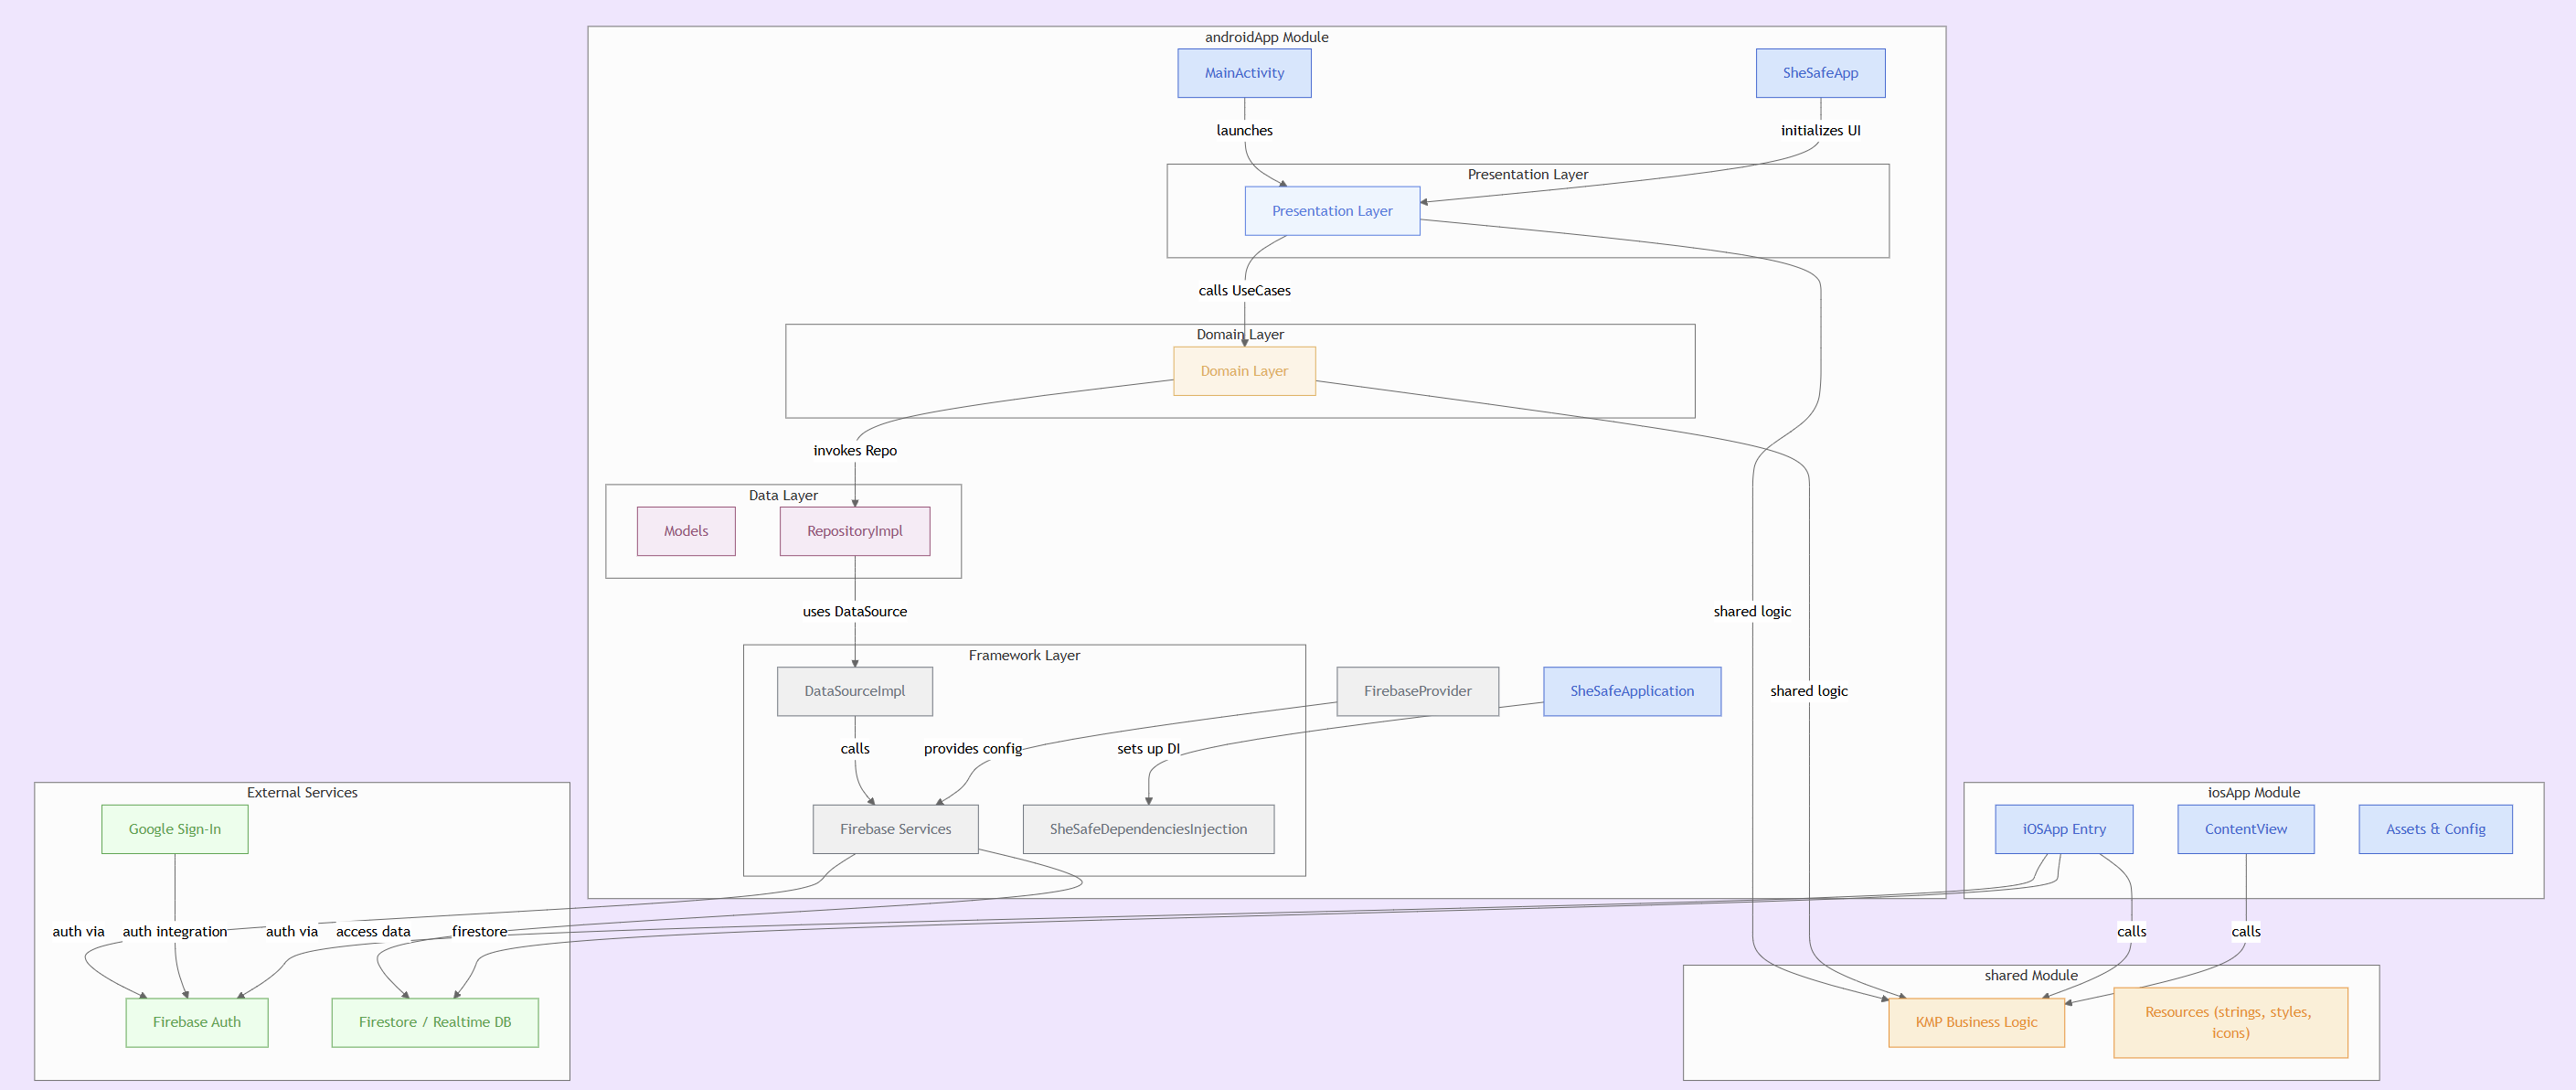
\includegraphics[width=0.8\linewidth]{images/shesafe/shesafe-architecture.png}\\
	\caption{Diagrama ilustrativo das camadas da Clean Architecture aplicada ao SheSafe}
	\label{fig:clean_architecture}
	\legend{Fonte: Próprio Autor}
\end{figure}
A estrutura de camadas implementada no projeto pode ser observada na organização dos pacotes dentro do módulo \texttt{androidApp}, conforme ilustrado na estrutura de diretórios do projeto:
\begin{figure}[H]
	\centering
	 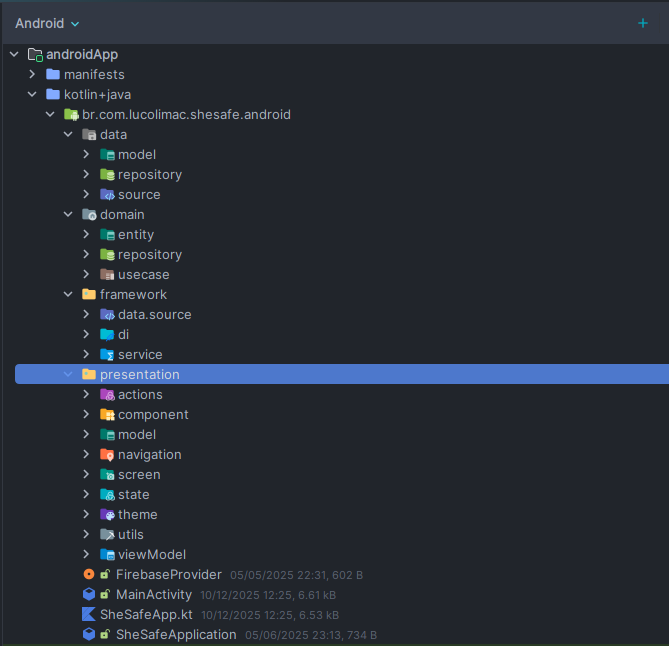
\includegraphics[width=0.8\linewidth]{images/shesafe/screenshot-clean-architecture-shesafe.png}\\
	\caption{Screenshot da estrutura de pastas do módulo androidApp mostrando os pacotes domain, data, framework e presentation}
	\label{fig:estrutura_pastas_androidapp}
	\legend{Fonte: Próprio Autor}
\end{figure}
\subsubsection{Camada de Domínio (Domain Layer)}
A camada de domínio representa o núcleo da aplicação, contendo as regras de negócio e entidades fundamentais do sistema. Esta camada é completamente independente de frameworks e tecnologias específicas, garantindo que a lógica de negócio permaneça isolada de detalhes de implementação. No projeto SheSafe, a camada de domínio está organizada no pacote \path{br.com.lucolimac.shesafe.android.domain} e compreende três subpacotes principais:

O subpacote \texttt{entity} contém as classes que representam os conceitos centrais do domínio da aplicação. As entidades \texttt{SecureContact} e \texttt{HelpRequest} encapsulam respectivamente as informações de contatos seguros cadastrados pelo usuário e os registros de pedidos de ajuda enviados. Estas entidades são classes de dados (\textit{data classes}) em Kotlin que implementam a interface \texttt{Parcelable}, permitindo sua serialização para passagem entre componentes Android. A entidade \texttt{HelpRequest} inclui lógica de domínio para geração de links do Google Maps baseados nas coordenadas de geolocalização, exemplificando como regras de negócio podem ser encapsuladas nas próprias entidades.

O subpacote \texttt{repository} define interfaces que especificam contratos para acesso a dados, sem se preocupar com os detalhes de implementação do armazenamento. As interfaces \texttt{SecureContactRepository}, \texttt{HelpRequestRepository}, \texttt{SettingsRepository}, \texttt{AuthRepository} e \texttt{HelpMessageRepository} declaram métodos para operações de leitura e escrita de dados, todas com modificador \texttt{suspend} indicando que são funções assíncronas executadas em corrotinas Kotlin. Esta abstração permite que a camada de domínio permaneça independente de decisões sobre qual tecnologia de persistência será utilizada, seja Firebase Firestore, banco de dados local ou qualquer outra solução.

O subpacote \texttt{usecase} implementa casos de uso da aplicação, representando as operações específicas que o sistema pode realizar. Cada caso de uso é definido por uma interface (como \texttt{SecureContactUseCase}, \texttt{HelpRequestUseCase}, \texttt{SettingsUseCase}, \texttt{AuthUseCase} e \texttt{HelpMessageUseCase}) e sua respectiva implementação (sufixo \texttt{Impl}). Os casos de uso orquestram a interação com repositórios e aplicam regras de negócio específicas, retornando dados através de \texttt{Flow}, uma construção de programação reativa do Kotlin que permite emissão assíncrona de valores. A implementação dos casos de uso utiliza \texttt{CoroutineDispatcher} configurado para \texttt{Dispatchers.IO}, garantindo que operações de I/O sejam executadas em threads apropriadas.

\subsubsection{Camada de Dados (Data Layer)}
A camada de dados atua como intermediária entre a camada de domínio e as fontes de dados externas, implementando os contratos definidos pelos repositórios e abstraindo os detalhes de acesso aos dados. Esta camada está organizada no pacote \path{br.com.lucolimac.shesafe.android.data} e subdivide-se em três componentes principais.

O subpacote \texttt{model} contém classes de modelo de dados (DTOs -- \textit{Data Transfer Objects}) que representam a estrutura dos dados conforme armazenados no Firebase Firestore. As classes \texttt{SecureContactModel} e \texttt{HelpRequestModel} incluem construtores vazios necessários para desserialização do Firestore, anotações \texttt{@SerializedName} do Gson para mapeamento de campos JSON, e métodos de conversão bidirecionais (\texttt{toEntity()} e \texttt{fromEntity()}) que transformam modelos de dados em entidades de domínio e vice-versa. Esta separação entre modelos de dados e entidades de domínio permite que mudanças na estrutura de armazenamento não afetem a lógica de negócio.

O subpacote \texttt{repository} fornece implementações concretas das interfaces de repositório definidas na camada de domínio. Classes como \texttt{SecureContactRepositoryImpl}, \texttt{HelpRequestRepositoryImpl}, \texttt{SettingsRepositoryImpl}, \texttt{AuthRepositoryImpl} e \texttt{HelpMessageRepositoryImpl} delegam operações para as respectivas fontes de dados, realizando conversões necessárias entre modelos e entidades. Estas implementações utilizam injeção de dependência para receber instâncias de \texttt{DataSource}, promovendo baixo acoplamento e facilitando testes unitários.

O subpacote \texttt{source} define interfaces abstratas de fontes de dados (\texttt{SecureContactDataSource}, \texttt{HelpRequestDataSource}, \texttt{SettingsDataSource}, \texttt{AuthDataSource} e \texttt{HelpMessageDataSource}) que especificam operações de acesso aos dados sem revelar detalhes de implementação específicos. Esta abstração adicional permite que diferentes implementações de armazenamento (Firebase, banco de dados local, API REST) sejam intercambiadas sem afetar as camadas superiores.

\subsubsection{Camada de Framework (Framework Layer)}
A camada de framework contém as implementações concretas que interagem diretamente com tecnologias e frameworks específicos, neste caso, o Firebase. Localizada no pacote \path{br.com.lucolimac.shesafe.android.framework}, esta camada materializa as abstrações definidas nas camadas superiores através de componentes específicos de infraestrutura.

O subpacote \texttt{service} contém interfaces de serviço e suas implementações Firebase. As interfaces \texttt{SecureContactService}, \texttt{HelpRequestService}, \texttt{SettingsService}, \texttt{AuthService} e \texttt{HelpMessageService} definem contratos para operações específicas, enquanto suas implementações (sufixo \texttt{FirebaseService}) realizam operações reais no Firestore e Firebase Authentication. Por exemplo, \texttt{SecureContactFirebaseService} utiliza a instância de \texttt{FirebaseFirestore} para acessar coleções específicas do usuário autenticado, implementando operações CRUD através da API assíncrona do Firebase com suporte a corrotinas Kotlin (\texttt{await()}).

O subpacote \texttt{data.source} fornece implementações concretas das interfaces \texttt{DataSource}, delegando operações para os serviços Firebase correspondentes. Classes como \texttt{SecureSecureContactDataSourceImpl}, \texttt{HelpRequestDataSourceImpl}, \texttt{SettingsDataSourceImpl}, \texttt{AuthDataSourceImpl} e \texttt{HelpMessageDataSourceImpl} tratam exceções e convertem resultados conforme necessário, atuando como adaptadores entre as abstrações da camada de dados e os serviços concretos do framework.

O subpacote \texttt{di} (\textit{Dependency Injection}) contém a configuração de injeção de dependências utilizando o framework Koin. O objeto \texttt{SheSafeDependenciesInjection} define o módulo Koin que registra todas as dependências do projeto, estabelecendo como instâncias de serviços, fontes de dados, repositórios, casos de uso e ViewModels devem ser criadas e injetadas. Esta configuração centralizada facilita a gestão de dependências e promove testabilidade através da possibilidade de substituir implementações reais por mocks durante testes.

\subsection{Padrão MVVM (Model-View-ViewModel)}
A camada de apresentação da aplicação adota o padrão arquitetural MVVM (\textit{Model-View-ViewModel}), amplamente recomendado para desenvolvimento Android por proporcionar separação clara entre lógica de apresentação e interface de usuário \cite{microsoft2023mvvm}. Este padrão facilita testes unitários da lógica de apresentação e permite que mudanças na interface não afetem a lógica subjacente.
\begin{figure}[htbp]
	\centering
	 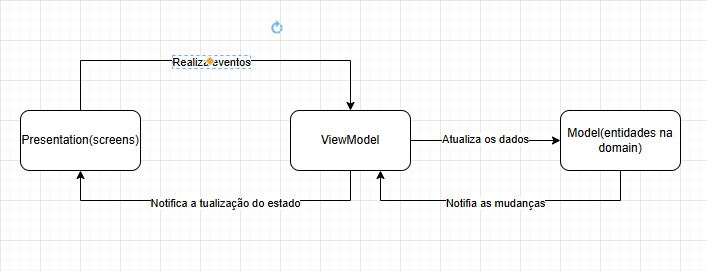
\includegraphics[width=0.8\linewidth]{images/shesafe/diagrama-mvvm.png}\\
	\caption{Diagrama ilustrando o fluxo de dados no padrão MVVM implementado no SheSafe}
	\label{fig:mvvm_fluxo}
	\legend{Fonte: Próprio Autor}
\end{figure}

\subsubsection{Camada de Apresentação (Presentation Layer)}
A camada de apresentação, localizada no pacote \path{br.com.lucolimac.shesafe.android.presentation}, organiza-se em diversos subpacotes especializados que implementam diferentes aspectos da interface de usuário e sua lógica associada.

O subpacote \texttt{viewModel} contém classes ViewModel que gerenciam o estado da interface e coordenam interações entre a View e a camada de domínio. Classes como \texttt{SecureContactViewModel}, \texttt{HelpRequestViewModel}, \texttt{SettingsViewModel}, \texttt{AuthViewModel}, \texttt{HomeViewModel} e \texttt{ProfileViewModel} estendem a classe base \texttt{ViewModel} do Android Architecture Components, garantindo que o estado da interface sobreviva a mudanças de configuração. Estas classes utilizam \texttt{StateFlow} e \texttt{Flow} para expor dados de forma reativa, permitindo que a interface observe mudanças de estado e se atualize automaticamente.

O subpacote \texttt{component} agrupa componentes reutilizáveis da interface de usuário construídos com Jetpack Compose. Componentes como \texttt{AppLogo}, \texttt{SearchBar}, \texttt{LastSentCard}, \texttt{SheSafeDialog}, \texttt{SheSafeBottomBar} e \texttt{SettingItem} encapsulam elementos visuais específicos que podem ser compostos para formar telas completas. Esta modularização promove reutilização de código e consistência visual em toda a aplicação.

O subpacote \texttt{navigation} implementa a estrutura de navegação da aplicação utilizando o Jetpack Navigation Compose. Define rotas de navegação como constantes (\texttt{HOME\_ROUTE}, \texttt{SECURE\_CONTACTS\_ROUTE}, \texttt{PROFILE\_ROUTE}, etc.) e fornece funções de extensão para o \texttt{NavController} que facilitam navegação entre telas. A classe \texttt{NavigationItem} representa itens do menu de navegação inferior, contendo informações sobre ícones e rotas associadas.

O subpacote \texttt{theme} define o sistema de design da aplicação através de arquivos que especificam cores (\texttt{Color.kt}), tipografia (\texttt{Typography.kt}), formas (\texttt{Shape.kt}) e o tema geral (\texttt{SheSafeTheme.kt}). Esta organização centralizada garante consistência visual e facilita ajustes globais no design da aplicação.

O subpacote \texttt{actions} contém classes que encapsulam ações complexas da interface, como \texttt{ScreenAction}, que implementa lógica para determinar qual tipo de diálogo deve ser exibido baseado no estado da aplicação (por exemplo, se há contatos seguros cadastrados).

O subpacote \texttt{model} define modelos específicos da camada de apresentação, como \texttt{DialogModel}, que encapsula informações necessárias para renderizar diálogos customizados, incluindo títulos, mensagens, textos de botões e callbacks para ações.

\section{Tecnologias e Frameworks}
\subsection{Jetpack Compose e Compose Multiplatform}
A interface de usuário da aplicação SheSafe foi desenvolvida utilizando Jetpack Compose, o toolkit moderno de UI declarativa do Android, e preparada para expansão multiplataforma através do Compose Multiplatform \cite{google2024compose}. Esta escolha tecnológica representa uma mudança paradigmática em relação ao desenvolvimento tradicional baseado em XML, oferecendo vantagens significativas em termos de produtividade, testabilidade e manutenibilidade.

O Jetpack Compose fundamenta-se no paradigma declarativo de construção de interfaces, onde o desenvolvedor descreve o estado desejado da UI através de funções composable, e o framework gerencia automaticamente a renderização e atualizações necessárias. Esta abordagem elimina a necessidade de manipulação imperativa de views e simplifica substancialmente o gerenciamento de estado da interface.

A estrutura do projeto demonstra preparação para desenvolvimento multiplataforma através da inclusão do módulo \texttt{shared} configurado com Kotlin Multiplatform. O arquivo \texttt{settings.gradle.kts} referencia explicitamente ambos os módulos (\texttt{androidApp} e \texttt{shared}), indicando a intenção de compartilhar código entre diferentes plataformas. O arquivo \texttt{build.gradle.kts} na raiz do projeto inclui plugins para \texttt{kotlinMultiplatform} e \texttt{jetbrainsCompose}, confirmando a configuração para suporte multiplataforma.

\begin{figure}[H]
	\centering
	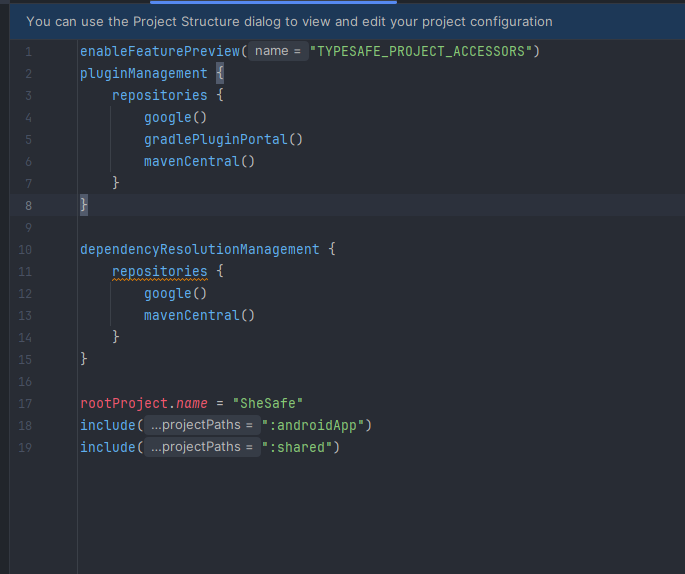
\includegraphics[width=0.8\linewidth]{images/shesafe/settings-gradle.png}\\
	\caption{Screenshot do arquivo settings.gradle.kts mostrando a inclusão dos módulos androidApp e shared}
	\label{fig:settings_gradle}
	\legend{Fonte: Próprio Autor}
\end{figure}
A adoção do Compose Multiplatform posiciona a aplicação para futura expansão para iOS e web, permitindo compartilhamento substancial de código de lógica de negócio e interface de usuário entre plataformas. Esta estratégia alinha-se com o objetivo de maximizar o alcance da ferramenta de proteção, disponibilizando-a para usuários independentemente da plataforma móvel utilizada.

\subsection{Firebase como Backend-as-a-Service}
A aplicação utiliza o Firebase como solução de backend-as-a-service, aproveitando múltiplos serviços da plataforma para diferentes funcionalidades. O Firebase Firestore atua como banco de dados NoSQL em tempo real, armazenando contatos seguros, pedidos de ajuda e configurações do usuário. O Firebase Authentication gerencia autenticação de usuários através do Google Sign-In. O Firebase Crashlytics monitora erros e crashes da aplicação em produção.

A inicialização do Firebase ocorre na classe \texttt{SheSafeApplication} através do método \texttt{FirebaseProvider.initialize()}, que configura as instâncias necessárias de \texttt{FirebaseAuth} e \texttt{FirebaseFirestore}. Estas instâncias são posteriormente injetadas nas classes de serviço através do Koin, promovendo testabilidade e desacoplamento.
\begin{figure}[H]
	\centering
	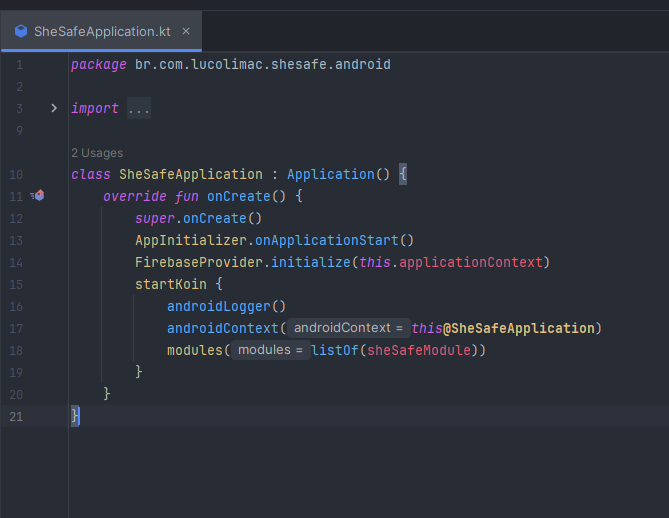
\includegraphics[width=0.8\linewidth]{images/shesafe/firebase-initializer.png}\\
		\caption{Screenshot da classe SheSafeApplication mostrando a inicialização do Firebase e do Koin}
	\label{fig:shesafe_application}
	\legend{Fonte: Próprio Autor}
\end{figure}
A estrutura de dados no Firestore organiza-se hierarquicamente, utilizando o email do usuário autenticado como identificador de documento principal. Por exemplo, contatos seguros são armazenados na coleção \texttt{secureContacts/[email]/contacts}, garantindo isolamento de dados entre diferentes usuários. Esta estrutura é implementada consistentemente em todos os serviços Firebase, como pode ser observado na classe \texttt{SecureContactFirebaseService}.
\subsection{Kotlin Coroutines e Flow}
A aplicação faz uso extensivo de Kotlin Coroutines para gerenciamento de operações assíncronas, evitando bloqueio da thread principal e garantindo responsividade da interface. Todas as operações de acesso a dados, desde chamadas ao Firestore até processamento de casos de uso, são implementadas como funções \texttt{suspend} que podem ser pausadas e retomadas sem bloquear threads.

A biblioteca Flow do Kotlin é utilizada para emissão reativa de dados, permitindo que observadores (como ViewModels) recebam atualizações automaticamente quando dados subjacentes mudam. Casos de uso retornam \texttt{Flow} de resultados, e ViewModels expõem \texttt{StateFlow} para que composables da interface observem mudanças de estado. Esta arquitetura reativa garante que a interface esteja sempre sincronizada com o estado mais recente dos dados.

O uso de \texttt{CoroutineDispatcher} configurado para \texttt{Dispatchers.IO} nas implementações de casos de uso garante que operações de I/O sejam executadas em pool de threads apropriado, otimizando performance e evitando sobrecarga da thread principal. Esta estratégia é observável em todas as classes de caso de uso, como \texttt{SecureContactUseCaseImpl}.

\subsection{Injeção de Dependências com Koin}
O projeto utiliza o framework Koin para injeção de dependências, configurando todas as dependências da aplicação no módulo definido em \texttt{SheSafeDependenciesInjection}. O Koin foi escolhido por sua simplicidade, integração nativa com Kotlin e performance adequada para aplicações Android.

A configuração do Koin utiliza DSL declarativa para registrar fábricas de instâncias, bindings de interfaces para implementações concretas, e ViewModels. A função \texttt{factoryOf()} cria novas instâncias sempre que solicitado, enquanto \texttt{viewModelOf()} registra ViewModels com escopo apropriado para sobreviver a mudanças de configuração. O método \texttt{bind<>()} estabelece mapeamento entre interfaces e implementações, permitindo que classes dependam de abstrações ao invés de implementações concretas.

\begin{figure}[H]
	\centering
	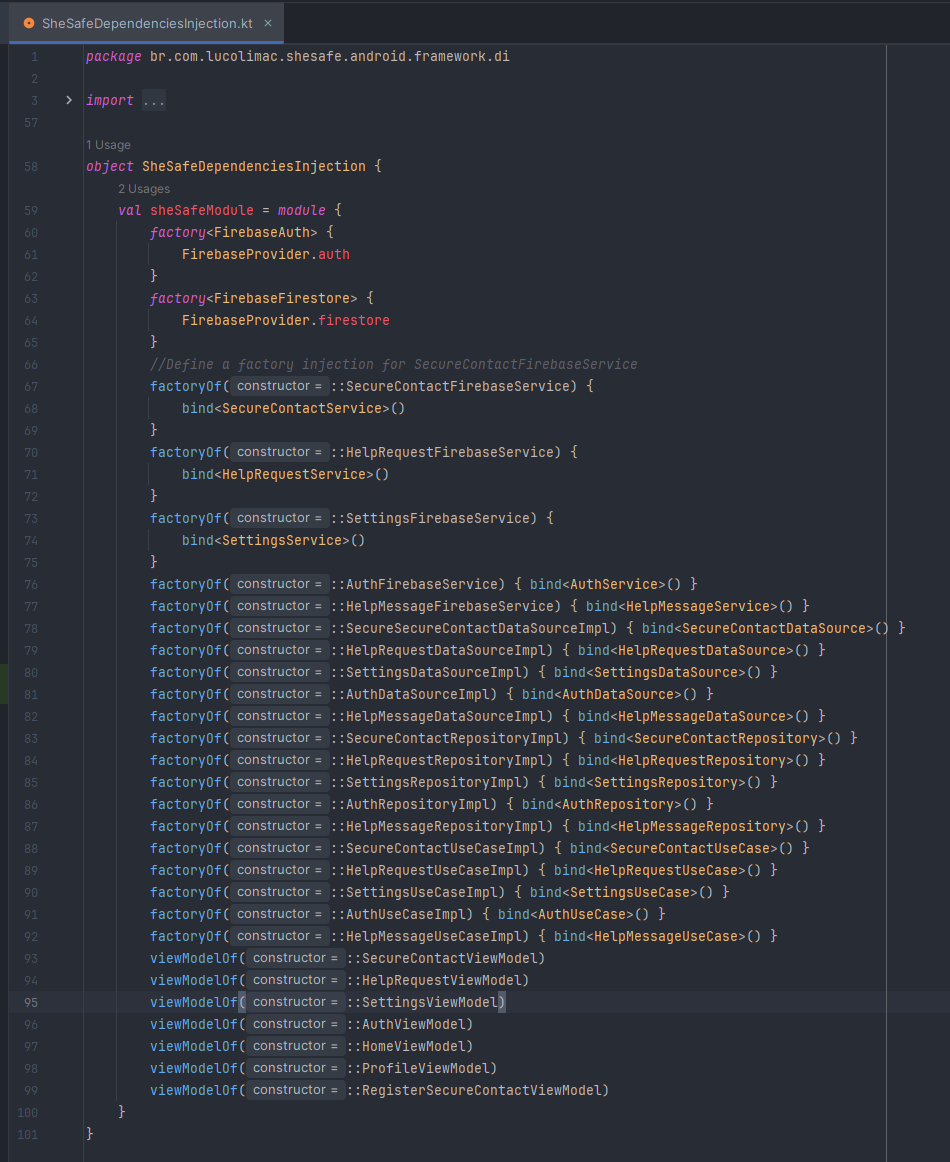
\includegraphics[width=0.4\linewidth]{images/shesafe/dependencie-injection.png}\\
	\caption{Screenshot da classe SheSafeDependenciesInjection mostrando a configuração do módulo Koin}
	\label{fig:koin_dependencies}
	\legend{Fonte: Próprio Autor}
\end{figure}
A inicialização do Koin ocorre em \texttt{SheSafeApplication.onCreate()}, onde o método \texttt{startKoin{}} configura o contexto Android e carrega o módulo de dependências. Esta configuração centralizada facilita manutenção e permite substituição de implementações para testes através de configuração de módulos alternativos.

\section{Funcionalidades Implementadas}
\subsection{Autenticação com Google Sign-In}
A aplicação implementa autenticação de usuários através do Google Sign-In, utilizando a biblioteca KMPAuth que fornece componentes Compose para integração com Firebase Authentication. A tela de login, implementada através do componente \texttt{SignInArea}, apresenta botão estilizado do Google que, ao ser clicado, inicia o fluxo de autenticação OAuth.

O resultado da autenticação é processado através de callback que recebe \texttt{Result<FirebaseUser?>}, permitindo tratamento apropriado de sucesso (navegação para tela principal) ou falha (exibição de mensagem de erro). Uma vez autenticado, o email do usuário é utilizado como identificador para organização de dados no Firestore, garantindo isolamento entre diferentes usuários.

A classe \texttt{AuthViewModel} gerencia o estado de autenticação, determinando qual deve ser a tela inicial da aplicação baseado em se há usuário autenticado. Esta verificação é implementada no método \texttt{isUserLoggedIn()} do \texttt{AuthUseCase}, que consulta \texttt{FirebaseAuth.currentUser} para determinar status de autenticação.

\subsection{Gerenciamento de Contatos Seguros}
A funcionalidade de gerenciamento de contatos seguros permite que usuários cadastrem, visualizem, editem e removam contatos que receberão alertas de emergência. A tela de listagem de contatos (\texttt{SecureContactsScreen}) apresenta lista de contatos cadastrados com opções de edição e remoção para cada item.

O cadastro de novos contatos é realizado através da tela \texttt{RegisterSecureContactScreen}, que apresenta formulário com campos para nome e número de telefone. A validação de dados garante que campos obrigatórios sejam preenchidos antes de permitir salvamento. A atualização de contatos existentes utiliza a mesma tela, pré-populando campos com dados atuais e alterando comportamento do botão de salvamento para executar operação de atualização ao invés de criação.

O \texttt{SecureContactViewModel} coordena operações relacionadas a contatos, mantendo estado da lista de contatos em \texttt{StateFlow} e expondo métodos para operações CRUD. Quando usuário solicita salvamento de contato, o ViewModel invoca caso de uso apropriado (\texttt{registerSecureContact} ou \texttt{updateSecureContact}), que por sua vez interage com repositório para persistir dados no Firestore.

\subsection{Envio de Pedidos de Ajuda}
A funcionalidade central da aplicação permite que usuários enviem pedidos de ajuda com geolocalização atual para todos os contatos seguros cadastrados. O botão de envio de ajuda, proeminentemente posicionado na tela principal (\texttt{HomeScreen}), ao ser pressionado, verifica primeiro se há contatos seguros cadastrados.

Caso não existam contatos cadastrados, diálogo é exibido oferecendo navegação direta para tela de cadastro de contato. Se contatos existem e configuração de confirmação está habilitada, diálogo de confirmação é apresentado antes de enviar pedido. Esta lógica é implementada na classe \texttt{ScreenAction} através do método \texttt{chooseDialogModel()}, que retorna modelo de diálogo apropriado baseado em estado da aplicação.

Ao confirmar envio, aplicação coleta localização atual do usuário através de APIs de geolocalização do Android, cria objeto \texttt{HelpRequest} contendo número de telefone do contato, coordenadas de localização e timestamp, e persiste este registro no Firestore. Simultaneamente, mensagem SMS é enviada para cada contato seguro contendo texto customizável pelo usuário e link do Google Maps apontando para localização exata.

O \texttt{HomeViewModel} orquestra este processo complexo, coordenando solicitação de permissões de localização e SMS (gerenciadas através do Accompanist Permissions), coleta de localização atual, formatação de mensagens, e invocação de casos de uso para persistência de dados e envio de mensagens.

\subsection{Visualização de Histórico de Pedidos}
A tela de histórico de pedidos (\texttt{HelpRequestsScreen}) apresenta lista cronológica de todos os pedidos de ajuda enviados pelo usuário, incluindo destinatário, localização e timestamp. Cada item da lista é renderizado através do componente \texttt{LastSentCard}, que exibe link clicável para visualização da localização no Google Maps.

O \texttt{HelpRequestViewModel} carrega lista de pedidos do repositório ao ser inicializado, expondo dados através de \texttt{StateFlow} observado pela interface. 
\begin{comment}
	A tela implementa pull-to-refresh para permitir que usuário atualize manualmente lista de pedidos, invocando novamente caso de uso de busca.
\end{comment}

\subsection{Configurações e Personalização}
A tela de configurações permite que usuários personalizem comportamento da aplicação, incluindo mensagem padrão enviada em pedidos de ajuda e opção de desabilitar diálogo de confirmação antes de enviar pedidos. O \texttt{SettingsViewModel} gerencia estado destas configurações, persistindo preferências no Firestore através do \texttt{SettingsRepository}.

A mensagem padrão é apresentada em campo de texto editável, com botão de salvamento que persiste alterações. A opção de confirmação é controlada através de switch que, ao ser alterado, atualiza imediatamente preferência no backend. Esta persistência em nuvem garante que configurações sejam mantidas mesmo se usuário trocar de dispositivo, desde que autentique com mesma conta Google.

\section{Considerações de Implementação}
\subsection{Tratamento de Permissões}
A aplicação requer permissões de localização (\texttt{ACCESS\_FINE\_LOCATION} e \texttt{ACCESS\_COARSE\_LOCATION}) e envio de SMS (\texttt{SEND\_SMS}) para funcionar adequadamente. O tratamento destas permissões é realizado utilizando a biblioteca Accompanist Permissions, que fornece componentes Compose para solicitação de permissões de forma declarativa.

Permissões são solicitadas em runtime no momento em que funcionalidade correspondente é acessada, seguindo melhores práticas do Android. Se usuário nega permissão, aplicação exibe explicação sobre necessidade da permissão e oferece opção de abrir configurações do sistema para concessão manual.

\subsection{Segurança e Privacidade}
A segurança dos dados é garantida através de regras de segurança do Firestore que restringem acesso aos dados de cada usuário. Apenas usuário autenticado pode acessar seus próprios dados, implementado através de regras que verificam correspondência entre \texttt{request.auth.uid} e identificador do documento.

A chave de API do Google Maps está exposta no arquivo \texttt{AndroidManifest.xml} para fins de desenvolvimento, mas deveria ser protegida através de variáveis de ambiente ou arquivo de configuração não versionado em produção. Credenciais do Firebase são gerenciadas através do arquivo \texttt{google-services.json}, que também deve ser protegido adequadamente.

\subsection{Qualidade de Código e Análise Estática}
O projeto utiliza Detekt, ferramenta de análise estática de código para Kotlin, configurada para aplicar regras de qualidade de código e detectar problemas potenciais. A configuração do Detekt está presente no arquivo \texttt{build.gradle.kts} raiz, especificando arquivo de configuração customizado e formatos de relatório (XML, HTML).

Esta análise automatizada ajuda a manter consistência de estilo, identificar code smells e garantir aderência a melhores práticas de desenvolvimento Kotlin. Relatórios gerados pelo Detekt podem ser integrados a pipelines de CI/CD para bloquear merges de código que violem regras estabelecidas.

O desenvolvimento da aplicação SheSafe fundamentou-se em princípios sólidos de engenharia de software, adotando arquiteturas e padrões consolidados que garantem manutenibilidade, escalabilidade e testabilidade do código. Este capítulo apresenta as decisões arquiteturais, tecnologias empregadas e a estrutura organizacional do projeto, demonstrando como a aplicação de conceitos teóricos de desenvolvimento de software materializou-se em uma solução tecnológica funcional.

\section{Avaliação com usuário}
A avaliação com usuário constitui-se como um paradigma metodológico fundamental no campo da Interação Humano-Computador (IHC), caracterizado pela participação direta de usuários reais no processo de análise e validação de sistemas interativos \cite{dix2003human}. Esta abordagem fundamenta-se no princípio de que a qualidade de um sistema deve ser mensurada a partir da perspectiva de quem efetivamente o utiliza, considerando suas necessidades, expectativas, limitações cognitivas e contextos de uso específicos \cite{preece2015interaction}.

Diferentemente dos métodos de inspeção realizados por especialistas, a avaliação com usuário oferece insights diretos sobre a experiência real de interação, revelando aspectos que podem não ser identificados através de análises teóricas ou heurísticas \cite{nielsen1994usability}. Esta metodologia permite a observação de comportamentos autênticos, identificação de estratégias de uso não previstas pelos designers, e compreensão das dificuldades reais enfrentadas pelos usuários em contextos naturais de utilização.
\subsection{Avaliação do usuário SheSafe}

As avaliações com usuário da aplicação SheSafe foram conduzidas ao longo do mês de setembro e outubro de 2025, envolvendo cinco participantes que executaram três tarefas específicas relacionadas às funcionalidades principais do sistema. Os testes foram realizados com a versão debug da aplicação Android, disponibilizada através de um link de download compartilhado com as avaliadoras.

Em relação ao cumprimento dos objetivos das tarefas, todas as participantes conseguiram completar as atividades propostas: enviar um pedido de socorro pela primeira vez, cadastrar um novo contato seguro e alterar a mensagem padrão do pedido de ajuda. Não foram registrados erros durante a execução de nenhuma das tarefas, indicando que a interface apresenta boa intuitividade e que os fluxos de interação estão adequadamente projetados para facilitar a conclusão das ações pelos usuários.

Na \autoref{tab:mediadetempo} é possível ver a média de tempo dos testes com os usuários para cada uma das três jornadas analisadas. Ela nos mostra uma performance satisfatória em todas as tarefas avaliadas. Para o envio do primeiro pedido de socorro, os tempos variaram entre 21 e 31 segundos, com média de 26,4 segundos. O cadastro de contatos seguros apresentou tempos mais consistentes, variando entre 13 e 18 segundos, com média de 15,6 segundos. A alteração da mensagem padrão apresentou tempos entre 11 e 25 segundos, com média de 17,2 segundos. Esta progressão temporal sugere que as funcionalidades mais críticas mantêm tempos de resposta adequados para situações de emergência, enquanto as funcionalidades de configuração apresentam variabilidade maior no tempo de execução.

\begin{table}[htbp]
	\centering
	\caption[Média de tempo de execução]{Média de tempo de execução}
	\label{tab:mediadetempo}
	\begin{tabular}{cc}
		\hline
		\multicolumn{1}{|c|}{Tarefa}                                        & \multicolumn{1}{c|}{Tempo médio}            \\ \hline \hline
		\multicolumn{1}{|c|}{Enviar um pedido de socorro pela primeira vez} & \multicolumn{1}{c|}{26,4s} \\ \hline
		\multicolumn{1}{|c|}{Cadastrar um novo contato seguro}              & \multicolumn{1}{c|}{15,6s} \\ \hline
		\multicolumn{1}{|c|}{Alterar a mensagem padrão do pedido de ajuda}  & \multicolumn{1}{c|}{17,2s} \\ \hline
	\end{tabular}
	\fonte{Próprio Autor}
\end{table}


No que se refere às impressões qualitativas, as avaliadoras expressaram percepções predominantemente positivas sobre diferentes aspectos da aplicação. A navegação foi consistentemente avaliada como adequada por todas as participantes, assim como o design visual e a usabilidade geral do sistema.
\begin{comment}
	Mônica Abreu destacou especificamente que "a interface é muito fácil e simples de aprender a utilizar", enquanto Wannielly Barbosa elogiou a "navegação fluida e sem problema para mudar de tela", caracterizando ainda a iniciativa como "ótima para mulheres".
\end{comment}

Contudo, emergiu um padrão consistente de feedback relacionado à ausência de confirmações explícitas do sistema após a execução de determinadas ações. Algumas das avaliadoras relataram especificamente a "falta de um retorno ao cadastrar o contato", enquanto uma outra observou que "ao alterar mensagem, só vi que alterou quando mudou na tela". Este feedback indica uma oportunidade de melhoria significativa no design de interação, particularmente na implementação de feedback imediato e explícito para ações críticas do usuário.

A convergência deste feedback específico sobre a ausência de confirmações do sistema sugere que esta deficiência pode impactar negativamente a confiança do usuário na aplicação, especialmente em um contexto de uso onde a certeza sobre a execução correta das ações é fundamental para a eficácia do sistema de segurança. A implementação de mensagens de confirmação, notificações toast, ou outros elementos de feedback visual imediato deveria ser considerada como prioridade para futuras iterações do desenvolvimento, visando aumentar a transparência do sistema e a confiança do usuário nas operações realizadas.